%; whizzy chapter
% -initex iniptex -latex platex -format platex -bibtex jbibtex -fmt fmt
% 以上 whizzytex を使用する場合の設定。

%     Kansai Debian Meeting resources
%     Copyright (C) 2007 Takaya Yamashita
%     Thank you for Tokyo Debian Meeting resources

%     This program is free software; you can redistribute it and/or modify
%     it under the terms of the GNU General Public License as published by
%     the Free Software Foundation; either version 2 of the License, or
%     (at your option) any later version.

%     This program is distributed in the hope that it will be useful,
%     but WITHOUT ANY WARRANTY; without even the implied warranty of
%     MERCHANTABILITY or FITNESS FOR A PARTICULAR PURPOSE.  See the
%     GNU General Public License for more details.

%     You should have received a copy of the GNU General Public License
%     along with this program; if not, write to the Free Software
%     Foundation, Inc., 51 Franklin St, Fifth Floor, Boston, MA  02110-1301 USA

%  preview (shell-command (concat "evince " (replace-regexp-in-string "tex$" "pdf"(buffer-file-name)) "&"))
% 画像ファイルを処理するためにはebbを利用してboundingboxを作成。
%(shell-command "cd image200708; ebb *.png")

%%ここからヘッダ開始。

\documentclass[mingoth,a4paper]{jsarticle}
\usepackage{kansaimonthlyreport}
\usepackage{ascmac}

% 日付を定義する、毎月変わります。
\newcommand{\debmtgyear}{2008}
\newcommand{\debmtgdate}{17}
\newcommand{\debmtgmonth}{8}
\newcommand{\debmtgnumber}{16}

\begin{document}

\begin{titlepage}

% 毎月変更する部分, 本文の末尾も修正することをわすれずに

 第\debmtgnumber{}回 関西 Debian 勉強会資料

\vspace{2cm}

\begin{center}
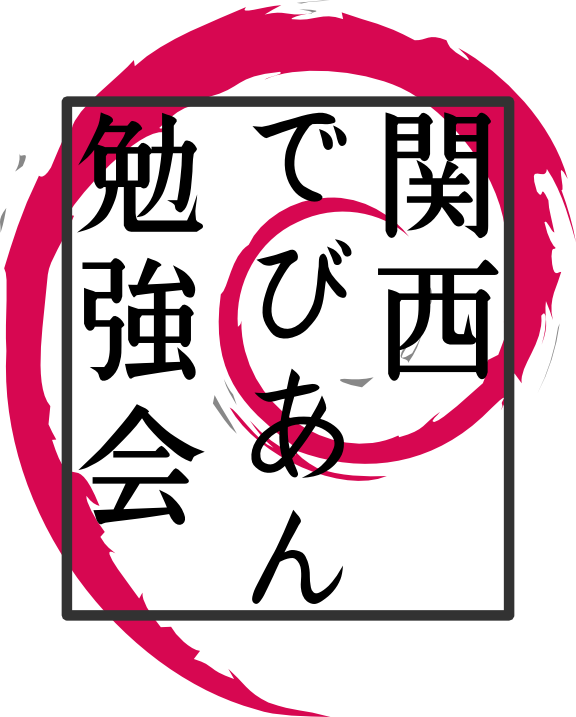
\includegraphics{image200802/kansaidebianlogo.png}
\end{center}

\begin{flushright}
\hfill{}関西 Debian 勉強会担当者 山下 尊也\\
\hfill{}\debmtgyear{}年\debmtgmonth{}月\debmtgdate{}日
\end{flushright}

\thispagestyle{empty}
\end{titlepage}

\dancersection{Introduction}{山下 尊也}
 
 関西 Debian 勉強会はDebian GNU/Linux のさまざ
 まなトピック(新しいパッケージ、Debian 特有の機能の仕組、Debian 界隈で起
 こった出来事、などなど)について話し合う会です。

 目的として次の三つを考えています。
 \begin{itemize}
  \item MLや掲示板ではなく、直接顔を合わせる事での情報交換の促進
  \item 定期的に集まれる場所
  \item 資料の作成
 \end{itemize}

 それでは、楽しい一時をお楽しみ下さい。

\newpage

\begin{minipage}[b]{0.2\hsize}
 {\rotatebox{90}{\fontsize{80}{80}
{\gt 関西デビアン勉強会}}}
\end{minipage}
\begin{minipage}[b]{0.8\hsize}
\hrule
\vspace{2mm}
\hrule
\setcounter{tocdepth}{1}
\tableofcontents
\vspace{2mm}
\hrule
\end{minipage}

\dancersection{最近のDebian関係のイベント報告}{山下 尊也}

\subsection{第14回 関西 Debian 勉強会}

2008年6月29日に「第14回 関西 Debian 勉強会」を福島区民センターにて行いました。
勉強会には、合計19名の方が参加しました。

\subsubsection{発表内容}

\begin{itemize}
 \item pbuilder でパッケージをビルドしてみる
 \item HotPlug の現状
 \item SSL のサーバー証明書が失効する時
\end{itemize}

懇親会は、阪神本線野田駅近くにある
「志な乃亭\footnote{\url{http://r.gnavi.co.jp/k029418/}}」にて行いました。
海鮮料理がおいしく、また、窓際の席だったため、阪神本線野田駅前の
交差点などをゆっくり見ながら、懇親会が出来たと思います。

また、懇親会にて、オープンソースカンファレンス2008 Kansaiにて
販売するのがたさん作Tシャツの先行販売が行われました。

\subsection{第15回 関西 Debian 勉強会}

2008年7月19日に「第15回 関西 Debian 勉強会」を行いました。
今回、資料としてまとめましたので、そちらをご覧下さい。

%% takaya
\dancersection{オープンソースカンファレンス2008 Kansai を振り返る}{山下 尊也} \label{sec:osckyoto}

関西 Debian 勉強会は、
7月19日に、京都コンピュータ学院京都駅前校にて行われました
オープンソースカンファレンス2008 Kansai
に参加しました。

イベント会場にて行ったものは、大きく分けて3つになります。
\begin{itemize}
 \item ブースにて配布したもの
 \item ブースにて販売したもの
 \item 関西 Debian 勉強会としてのセッション「第15回 関西 Debian 勉強会」
\end{itemize}

これらを含めた上で、今後、関西 Debian 勉強会がオープンソースカンファレンス
(以下:OSC)などのイベントに参加する時、
どのように行っていけば良いのか検討したいと思います。

\subsection{配布したもの}

今回、ブースにて配布したものは以下のものです。

\begin{itemize}
 \item 勉強会のポストカード
 \item Debian Live DVD\footnote{Software Design 2008 年 8 月号「Debian
       live-helper」
       \url{http://gihyo.jp/magazine/SD/archive/2008/200808}に Debian JP
       Project の岩松さん担当しました記事がありますので、そちらもご覧下
       さい。}
\end{itemize}

A4の紙で勉強会について説明した紙を配布すると、
他のブースと紙のサイズが同じになるため
インパクトが弱くなります。
そのため、ポストカードを採用しました。
また、ポストカードを採用したため、A4のカラー印刷に比べ、
印刷にかかる費用を抑える事が出来ました。

また、昨年の関西オープンフォーラム(以下:KOF)や前回の
OSCの際は、
Debian Installer のマルチアーキテクチャーを配布していましたが、
1DVD Linuxとしても使える Debian Live DVDを配布しました。
この DVDを用いてDebianのインストールを行う事も出来ます。

\subsection{販売したもの}

\begin{minipage}{0.5\hsize}
% \begin{table}[htbp]
%  \caption{販売価格}
\begin{center}
 \begin{tabular}{|c|c|}
  \hline
  品目 & 値段 \\ \hline
  あんどきゅめんてっど でびあん
  \footnote{有志で紙媒体に印刷して有償で配布していますが\url{http://tokyodebian.alioth.debian.org/undocumenteddebian.html}にてPDF形式でも配布しています。} & 1冊1000円 \\ \hline
  Tシャツ & 1着2000円 \\ \hline
  のがたさん作のシール & 5枚100円 \\ \hline
  岩松さん作のシール & 1枚200円 \\ \hline
 \end{tabular} 
\end{center}
%  \label{tb:sale}
% \end{table}
\end{minipage}
\begin{minipage}{0.5\hsize}
%\begin{figure}[htbp]
 \begin{center}
  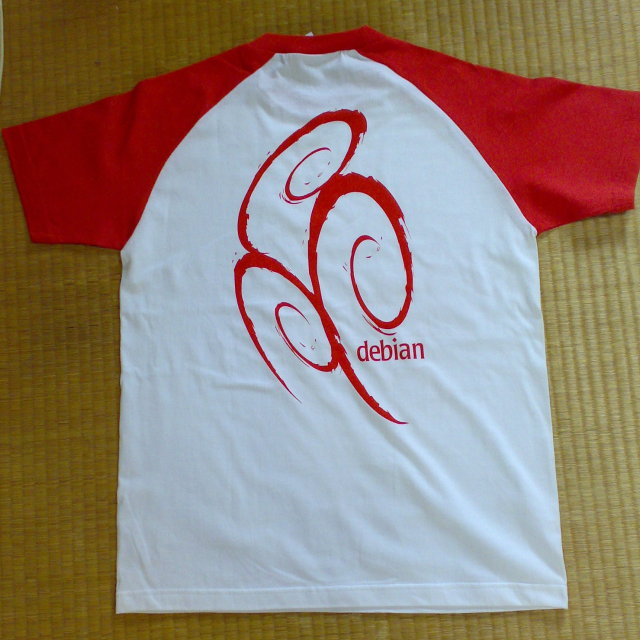
\includegraphics[height=50mm]{image200808/t-shirts.jpg}
 \end{center}
% \caption{販売したTシャツ}
% \label{fig:t-shirts}
%\end{figure}
\end{minipage}

\hspace{5mm}

岩松さんから私に届いたシールとのがたさん作のシールの違いは、
岩松さんのシールがカッティングシールになっていたため、
販売する値段に差があります。

今回のイベントでの売上についてですが、表\ref{tb:sales}にまとめました。
合計で32200円の売上になりましたが、
ブースとして必要になった金額(17285円)を引いた
金額(14915円)を Debian JP Project に寄付させて頂きました。
\footnote{Debian JP Projectでは、ミラーサーバなどサービス向上を図るため
に、皆様からの寄付をお待ちしております。詳しくは、
\url{http://www.debian.or.jp/project/donations.html}をご覧下さい。}

\begin{table}[htbp]
\caption{今回のイベントでの売上}
\begin{center}
\begin{tabular}{|l|r|r|r|}
\hline
 & \multicolumn{1}{l|}{単価} & \multicolumn{1}{l|}{個数} & \multicolumn{1}{l|}{合計} \\ \hline
Tシャツ(M) & 2000 & 10 & 20000 \\ \hline
Tシャツ(L) & 2000 & 6 & 12000 \\ \hline
ステッカー(のがた) & 100 & 2 & 200 \\ \hline
売上総計 & \multicolumn{1}{l|}{} & \multicolumn{1}{l|}{} & 32200 \\ \hline 
\end{tabular}
\end{center}
\label{tb:sales}
\end{table}

また、販売したTシャツについても東京エリア Debian 勉強会が
OSC 2008 Tokyo/Wall\footnote{\url{http://www.ospn.jp/osc2008-fall/}}に
参加する予定ですので、MサイズとLサイズをそれぞれ5着送らせて頂きました。

\subsection{ライトニングトーク}

関西 Debian 勉強会では、OSC などのイベント会場にて、普段行っている勉強会
と同じ内容のものを開催したいと考えて来ましたが、部屋の確保出来る時間の問題や講
師側の問題もあり、ライトニングトークで行う事にしました。

\begin{itemize}
 \item EeePC with SSD に Debian をインストールして設定してみた
 \item ある1ユーザから見た Debian
 \item Debian Live やろうぜ
 \item developer news 翻訳の舞台裏
 \item DebianLive で Ubuntu 風インストール画面を夢見る
\end{itemize}

一部のライトニングトークで行った内容につきましては、今後の勉強会にて
講師をして頂きたいと考えています。

\newpage

\subsection{イベント終了後}

交通の利便性も考え、京都駅近くで懇親会を行うことにしました。

JR京都駅八条口から徒歩1分にあります
「焼肉の寿々\footnote{\url{http://www.h4.dion.ne.jp/~juju/index.htm}}」
にて関係者の懇親会を行いました。

関係者の中から、「OSCの懇親会にも
参加したかった」と声があったため、今後は、懇親会をどのように行うかについても、関係者メーリングリストなどで、改めてアンケートなどをとりたいと思います。

\subsection{今後改善すべき点}

\subsubsection{全体として}

\begin{itemize}
 \item OSC に出展する意義を周知・統一しておくべき
       \begin{itemize}
	\item 関西Debian勉強会を広めるのか?それともDebianを広げるのか?
       \end{itemize}
 \item セミナーの練習が必要だった
 \item セミナーとブースについてアンケートを実施した方が良い
 \item 一部の人がOSCのメーリングリストには入っているが、連絡事項について周知出来ていない点が多かった
       \begin{itemize}
	\item 貼り付け用の両面テープは受付(事務局)で配布するなどの注意事
	      項
	\item ブースは、テーブルの半分のスペース
       \end{itemize}
 \item 負担が一定の人に集中し過ぎていた
 \item 関西 Debian 勉強会が、Debian勉強会ではなくて、ただのユーザーグルー
       プになっている可能性
 \item OSC運営側にも参加する
       \begin{itemize}
	\item ブースの大きさなど意見を出す
       \end{itemize}
 \item Ubuntu Japanese Teamと共同で何かイベントを開催する
\end{itemize}

\subsubsection{ブースについて}

\begin{itemize}
 \item 会場の設置の際に使った両面テープが強力過ぎて、跡を残さないように
       剥がすのが大変だった
       \begin{itemize}
	\item 窓ガラスに両面テープを貼らない
	\item 壁がガラスの会場が多いため、ゴム吸盤が確実
       \end{itemize}
 \item ポストカードサイズにするなら、はがきとして使えるデザインに
       する
 \item POPをもっと大きいものにする
 \item 服を売る際は、ハンガーがあった方がよい
 \item どんな活動をしているかが、外から見えなかった
       \begin{itemize}
	\item 関西*BSDユーザ会のように、最近の活動内容をお品書き風に書く
	\item 活動風景の写真をPCに表示するのもいいかもしれない
       \end{itemize}
 \item ブーススタッフの人数が十分確保できそうな場合は、人数を決めておく
       べき
       \begin{itemize}
	\item 2人ぐらいがベスト?
	\item 組み合わせなども考慮した方が良い
	\item スタッフの数が多いと、机の前に大量に占拠してしまう
	\item スタッフルームに、関西 Debian 勉強会のメンバーが溜まってい
	      た
	\item スタッフルームにて、私事をする人がいた
       \end{itemize}
\end{itemize}

%% namura
\dancersection{DebianをWindowsなPCでも楽しもう --応用編}{名村 知弘}
\label{sec:colinux}

\subsection{はじめに}
coLinuxの配布サイト
\footnote{\url{http://sourceforge.net/projects/colinux/files}}では、
Debian etchのイメージファイルが配布されていますので、
coLinuxをインストールすると、すぐにDebianを楽しむことができます。

しかし、配布されているイメージファイルは、
ディスクイメージのサイズが1GBだったり、
どのようなパッケージがどういった設定でセットアップされているのかなど、
中身が非常に気になったりします。

ダウンロードすればお手軽に使えるというのは良いのですが、
将来の拡張のためパーティション構成を変更したり、
イメージの内容をいちいち確認するのも面倒ですし、
それならばいっその事、新規インストールしてみよう。
と言うことで、半ば強引な導入ですが、
coLinuxにDebianを新規インストールする方法と、
coLinuxにインストールされたXアプリケーションを起動する方法をご紹介します。

説明するにあたり、以下の前提で記載していますので、
適宜それぞれの環境に応じて読み替えていただくようお願いいたします。
\begin{enumerate}
\item coLinuxを\verb|c:\coLinux|にインストールしているものとしています。
\item coLinuxはネットワーク共有にて接続されているものとしてます。
\item Debianはetchを使用するものとしています。
\item DebianはIPアドレス192.168.0.10が割り当てられているものとしています。
\end{enumerate}

\subsection{coLinuxにDebianを新規インストール}
coLinuxへのDebianインストール手順は以下のようになります。
\begin{enumerate}
\item Debianをインストールするためのディスクイメージの作成
\item DebianのISOイメージを入手
\item initrdイメージの取得
\item coLinuxをDebianインストール用に設定
\item Debianのインストール
\item coLinuxを通常起動用に設定
\end{enumerate}



\subsubsection{Debianをインストールするためのディスクイメージの作成}
coLinuxでは、1つのパーティションに対して1つのディスクイメージファイルを用意することで、
HDDをエミュレートしています。
ディスクイメージファイルはあらかじめ必要なサイズを割り当てる必要があり、
coLinuxが割り当てられたサイズを超えて書き込むことはできません。
(つまり、HDDが一杯になったら書き込めないのと同様、
ディスクイメージファイルに割り当てられたサイズを使用すると、それ以上書き込みが行えなくなります)

今回は以下の構成でインストールを行いたいと思います。
\begin{table}[htbp]
\begin{center}
  \begin{tabular}[htbp]{|l|l|l|}\hline
    領域 & サイズ & ディスクイメージ\\ \hline\hline
    / & 2GB & \verb|root_fs|\\ \hline
    /home & 2GB & \verb|home_fs|\\ \hline
    swap & 500MB & \verb|swap_fs|\\ \hline
  \end{tabular}
  \caption{パーティション割り当て}
  \label{tab:colinux_partition}
\end{center}
\end{table}

ここでは3パーティション使用するため、3ファイル作成する必要があります。
また、あらかじめ使用するサイズを割り当てる必要があるため、
Windowsのfsutilコマンドを使用します。
fsutilは指定されたファイル名、サイズで空ファイルを作成することができます。

ファイル名とサイズは表\ref{tab:colinux_partition}に基づいて決定していますので、
お手持ちのPCのディスク空き容量などを考慮しながら、
適切なサイズを決定していただければと思います。

コマンドプロンプトを起動し、\verb|c:\coLinux|にcdしてから、
以下のコマンドを実行するとファイルが作成されます。

\begin{commandline}
fsutil file createnew root_fs 2147483648
fsutil file createnew home_fs 2147483648
fsutil file createnew swap_fs 536870912
\end{commandline}

\subsubsection{DebianのISOイメージを入手}
まずはDebianをインストールするための、ISOイメージを入手
\footnote{\url{http://www.debian.org/CD/netinst/}}します。
ここではdebian-40r4a-i386-businesscard.isoを使用します。

\subsubsection{initrdイメージの取得}
\verb|c:\coLinux|には、
coLinux起動用のinitrdイメージが用意されていますが、
Debianインストール用にcoLinuxを起動するためには、
インストール用に起動するためのinitrdイメージが必要となります。

インストール起動用と通常起動用のinitrdイメージを混同してしまわないように、
\verb|c:\coLinux|にあるオリジナルのinitrd.gzを、
initrd-normal.gzとリネームしておきます。

インストール用のinitrdイメージは、DebianのISOイメージに収録されているため、
ISOイメージを展開できるツール、Explzh\footnote{\url{http://www.ponsoftware.com/archiver/}}や、
TUGZip\footnote{\url{http://www.tugzip.com/}}を使用して取り出します。

展開ツールをインストールして起動し、DebianのISOイメージを開きます。
ISOイメージの中の、「/install.386/initrd.gz」を取り出し、
こちらも通常起動用のinitrdイメージと混同してしまわないように、
initrd-install.gzとリネームして、\verb|c:\coLinux|に保存します。


\subsubsection{coLinuxをDebianインストール用に設定}
coLinuxをインストール用に起動するためのファイルは全て揃いましたので、
これらファイルを使用してDebianインストールが行われるよう、
coLinuxの設定を変更します。

\verb|c:\coLinux|にdebian-install.confと言う名前でファイルを作成し、
以下の内容を記載して保存します。

\begin{commandline}
kernel=vmlinux
initrd=initrd-install.gz
mem=512
cobd0="\DosDevices\C:\coLinux\swap_fs"
cobd1="\DosDevices\C:\coLinux\root_fs"
cobd2="\DosDevices\C:\coLinux\home_fs"
cobd3="\DosDevices\C:\coLinux\debian-40r4a-i386-businesscard.iso"
cofs0="\DosDevices\C:\coLinux"
eth0=tuntap
root=/dev/cobd1
ro
\end{commandline}

上記設定ファイルを簡単に説明すると、
2行目でインストール起動用のinitrdイメージを指定し、
3行目でcoLinuxの使用するメモリサイズを指定します。
4〜6行目で使用するディスクイメージ(今回は3つ)を指定します。
7行目でDebianのISOイメージを指定します。
8行目でcoLinuxインストールディレクトリを指定します。
10行目で「/」ファイルシステムのデバイス名を指定します。

\subsubsection{Debianのインストール}
準備が整いましたので、debian-install.confを使用してcoLinuxを起動します。
コマンドプロンプトを起動し、\verb|c:\coLinux|にcdしてから、
以下のコマンドを実行します。

\begin{commandline}
colinux-daemon.exe -t nt "@c:\coLinux\debian-install.conf"
\end{commandline}

そうすると、いつもの見慣れた?インストール画面が起動されますので、
以下の手順に従ってインストールを進めていきます。

まずはインストーラの環境設定を行います。
以下の手順に従ってインストール作業を進めていきます。

\begin{commandline}
# インストーラで使用する言語を選択します。
* English (Japaneseではインストール中に表示されるメッセージが文字化けします)

# 国を選択します。
* Japan ( <other> → <Japan> )

# キーマップを選択する。
* Japanese (ご使用のキーボードに合わせてください)

# CD-ROMのドライバはcoLinuxが設定してくれるため必要ありません。
* <No>

# CD-ROMのドライバはcoLinuxが設定してくれるため、手動で使わないよう設定します。
* <Yes>→「none」
\end{commandline}

ここまで実行すると、図\ref{fig:colinux_cdrom}のような、CD-ROMをマウントする画面が表示されます。

\begin{figure}[htbp]
 \begin{center}
  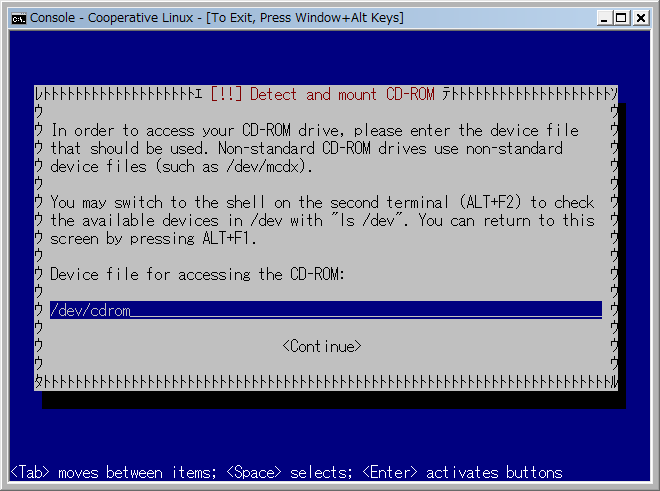
\includegraphics[width=100mm]{image200808/colinux_cdrom.png}
 \end{center}
 \caption{CD-ROMのマウント}
 \label{fig:colinux_cdrom}
\end{figure}

しかし、インストーラはcoLinuxが設定してくれたCD-ROMドライブにアクセスするためのデバイスファイルを
作成していないため、このままではCD-ROMにアクセスすることができません。

そこで、coLinuxが設定してくれた各種デバイスにアクセスするための、
デバイスファイルを作成します。

[ALT] + [F2] キーを押し、インストーラ画面からターミナルに移動します。
移動すると、図\ref{fig:colinux_secound_console}のような画面が表示されます。

\begin{figure}[htbp]
 \begin{center}
  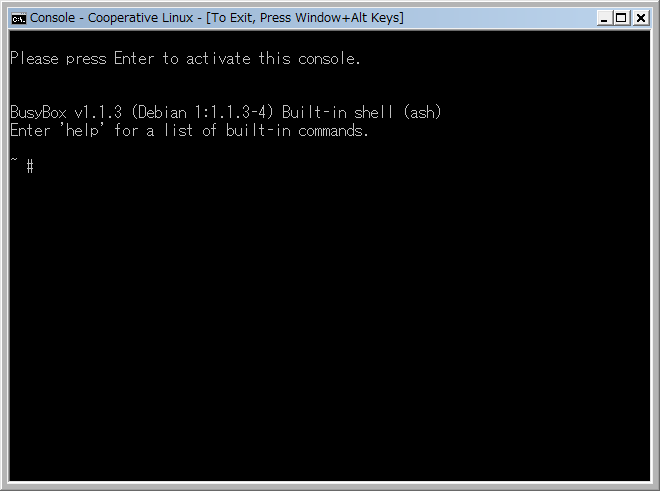
\includegraphics[width=100mm]{image200808/colinux_secound_console.png}
 \end{center}
 \caption{ターミナルに移動}
 \label{fig:colinux_secound_console}
\end{figure}

ターミナルにて以下のコマンドを入力します。

\begin{commandline}
# デバイスファイル/dev/cobdxを作成します。
i=0; while [ $i -lt 32 ]; do mknod /dev/cobd$i b 117 $i; i=`expr $i + 1`; done

# 環境によっては「mknod: /dev/cobdx: File exists」と言うメッセージが表示されることがありますが、
# これは既に/dev/cobdxが作成されているということですので、
# そのまま次に進めてもらっても問題ありません。

# デバイスファイル/dev/cofsxを作成します。
i=0; while [ $i -lt 16 ]; do mknod /dev/cofs$i b 117 $i; i=`expr $i + 1`; done
\end{commandline}

これでcoLinuxが設定してくれたCD-ROMをマウントすることができるようになりましたので、
[ALT] + [F1] キーを押し、ターミナルからインストーラ画面に戻ります。
戻ると、先程中断した図\ref{fig:colinux_cdrom}の画面が表示されますので、
以下の手順に沿ってインストール作業を進めていきます。

\begin{commandline}
# CD-ROMをマウントするため、DebianのISOイメージが設定されているデバイスファイルを指定します。
# 今回はdebian-install.confの7行目にて以下のように設定していますので、「/dev/cobd3」を指定します。
# cobd3="\DosDevices\C:\software\coLinux\debian-40r1-i386-businesscard.iso"
* 「/dev/cobd3」と入力し<Continue>

# カーネルモジュールはcoLinuxのものを使用しますので、読み込まずにインストールを続けます。
* <Yes>

# ネットワークを設定が行われますが、Windows側で設定が済んでいればDHCPで取得できますので、
# 特に何かする必要はありません。
\end{commandline}

ネットワークの設定が終わると、以降のインストールはDebianのインストールでは行えませんので、
続きの作業は手動にて行っていきます。

[ALT] + [F2] キーを押し、再びターミナルに移動し、
以下のコマンドを順次実行していきます。

\begin{commandline}
# まずはswapファイルを作成し、有効化します。
# 今回はdebian-install.confの4行目にて以下のように設定していますので、
# 「/dev/cobd0」に対してmkswapを実行します。
# cobd0="\DosDevices\C:\software\coLinux\KDM#16\swap_fs"
mkswap /dev/cobd0
sync; sync; sync
swapon /dev/cobd0

# 次に、coLinuxをインストールするために用意したディスクイメージに
# ext3ファイルシステムを作成します。
# 今回はdebian-install.confの5, 6行目にて以下のように設定していますので、
# 「/dev/cobd1」、「/dev/cobd2」に対してmke2fsを実行します。
# cobd1="\DosDevices\C:\software\coLinux\KDM#16\root_fs"
# cobd2="\DosDevices\C:\software\coLinux\KDM#16\home_fs"
mke2fs -j /dev/cobd1
mke2fs -j /dev/cobd2

# インストール対象の「/」をマウントするためのディレクトリを作成し、マウントします。
mkdir /target
mount /dev/cobd1 /target
cd /target

# coLinux附属のカーネルモジュールを使用するため、\verb|c:\coLinux|をマウントし、
# \verb|c:\coLinux\vmlinux-modules.tar.gz|を/targetに展開します。
mkdir -p /mnt/windows
mount -t cofs /dev/cofs0 /mnt/windows
tar -zxvf /mnt/windows/vmlinux-modules.tar.gz

# /targetにcoLinuxの設定するデバイスファイルを作成します。
mkdir /target/dev
i=0; while [ $i -lt 32 ]; do mknod /target/dev/cobd$i b 117 $i; i=$((i+1)); done
i=0; while [ $i -lt 16 ]; do mknod /target/dev/cofs$i b 117 $i; i=$((i+1)); done

# /targetにetcディレクトリを作成し、各種設定ファイルを作成しておきます。
mkdir /target/etc

# HTTPプロキシが必要な環境に接続されている場合、プロキシの設定を行います。
export http_proxy=http://myproxy.co.jp:8888

# debootstrapにて最小構成のDebianディレクトリツリーを作成します。
# ここではetchを指定していますが、sidやlennyを指定することもできます。
debootstrap --arch i386 etch /target http://cdn.debian.or.jp/debian/

# /targetにchrootし、インストール環境を設定していきます。
chroot /target

# /target/etc/fstabにインストール後のマウント情報を作成します。
cat <<EOF > /etc/fstab
/dev/cobd0 swap  swap defaults 0 0
/dev/cobd1 /     ext3 defaults 1 1
/dev/cobd2 /home ext3 defaults 1 1
proc       /proc proc defaults 0 0
EOF

# ネットワーク関連を設定します。
# お使いのcoLinuxの設定に合わせて行ってください。
cat <<EOF >> /etc/network/interfaces
auto lo
iface lo inet loopback
auto eth0
#iface eth0 inet dhcp
iface eth0 inet static
  address 192.168.0.10
  netmask 255.255.255.0
  gateway 192.168.0.1
EOF

echo "nameserver 192.168.0.1" > /etc/resolv.conf

echo "coLinux" > /etc/hostname

cat <<EOF >> /etc/hosts
127.0.0.1      localhost
192.168.0.10   coLinux
EOF

ln -sf /usr/share/zoneinfo/Japan  /etc/localtime

# shadowパスワードを有効にします
shadowconfig on

# aptリポジトリを設定します。
# ここではetchを指定していますが、sidやlennyを指定することもできます。
cat <<EOF > /etc/apt/sources.list
deb http://cdn.debian.or.jp/debian etch main contrib non-free
deb-src http://cdn.debian.or.jp/debian etch main contrib non-free
EOF

# ロケーション関連を設定します。
aptitude update
aptitude -y install console-common
dpkg-reconfigure console-data

aptitude -y install locales
dpkg-reconfigure locales
\end{commandline}

これで基本となるインストール作業は完了したため、
Debianインストーラを終了させます。

[ALT] + [F1] キーを押し、ターミナルからインストーラ画面に移動し、
以下の手順に従ってインストーラを終了させます。

\begin{commandline}
# Debianインストーラを終了させます。
[ESC]キーを押下し、ネットワーク設定画面に戻ります。
もう一度[ESC]キーを押下し、メインメニューに戻ります。
メニュー一番下の「Abort the installation」を選択し[Enter]を押下します。
* <Yes>
\end{commandline}
これでcoLinuxが再起動されますが、設定ファイルがインストール起動用となっているため、
再びDebianインストーラが起動されますので、一旦coLinuxを終了させます。

\subsubsection{coLinuxを通常起動用に設定}
coLinuxへのDebianインストールは完了しましたので、
通常起動するためにcoLinuxの設定を変更します。

coLinuxインストールディレクトリにdebian.confと言う名前でファイルを作成し、
以下の内容を記載して保存します。

\begin{commandline}
kernel=vmlinux
initrd=initrd-normal.gz
mem=512
cobd0="\DosDevices\C:\software\coLinux\kdm\swap_fs"
cobd1="\DosDevices\C:\software\coLinux\kdm\root_fs"
cobd2="\DosDevices\C:\software\coLinux\kdm\home_fs"
eth0=tuntap
root=/dev/cobd1
ro
\end{commandline}

あとは、この設定ファイルを使用してcoLinuxを起動すると、
先程インストールしたオリジナルイメージで起動することができます。
コマンドプロンプトを起動し、\verb|c:\coLinux|にcdしてから、
以下のコマンドを実行します。

\begin{commandline}
colinux-daemon.exe -t nt "@c:\coLinux\debian.conf"
\end{commandline}



\subsection{XmingによるXアプリケーション起動方法}
coLinuxにはディスプレイデバイスが実装されていないため、
そのままではCUI環境でしか使用することができません。
しかし、XサーバやVNC、sshのX11フォワードなどの機能を使用すると、
Xアプリケーションを使用することができます。

今回はXmingを使用した、sshのX11フォワードとXDMCPについて紹介したいと思います。

sshのXフォワードでは必要ないのですが、XDMCP接続では、
ログインマネージャを使用する必要がありますので、
ログインマネージャとしてGDMを使用したXDMCP接続について説明したいと思います。

大まかな手順は以下のようになります。
\begin{enumerate}
\item Xmingのインストール
\item Xアプリケーションのインストール
\item sshのXフォワードで起動
\item XDMCPで起動
\end{enumerate}


\subsubsection{Xmingのインストール}
Xmingの配布サイト\footnote{\url{http://sourceforge.net/projects/xming/files}}から、
Xmingのインストーラ\footnote{執筆時ではXming-6-9-0-31-setup.exeが最新版となっています}と
コアXフォントのインストーラ\footnote{執筆時ではXming-fonts-7-3-0-22-setup.exeが
最新版となっています}をダウンロードし、インストールします。


\subsubsection{Xアプリケーションのインストール}
起動するXアプリケーションのインストールを行います。
ここではiceweaselをサンプルとして起動してみたいと思いますので、
iceweaselをインストールしておきます。

また、XDMCPで起動する方法もご紹介いたしますので、
XDMCP接続時のログインマネージャとしてGDMをインストールします。

\begin{commandline}
sudo aptitude install ssh gdm iceweasel
\end{commandline}

GDMをインストールすると、Debian起動時にGDMが起動しようとするのですが、
ディスプレイデバイスを持たないcoLinuxではGDM起動に失敗してしまい、
図\ref{fig:colinux_gdmerror}のようなエラー画面が表示されます。

\begin{figure}[htbp]
 \begin{center}
  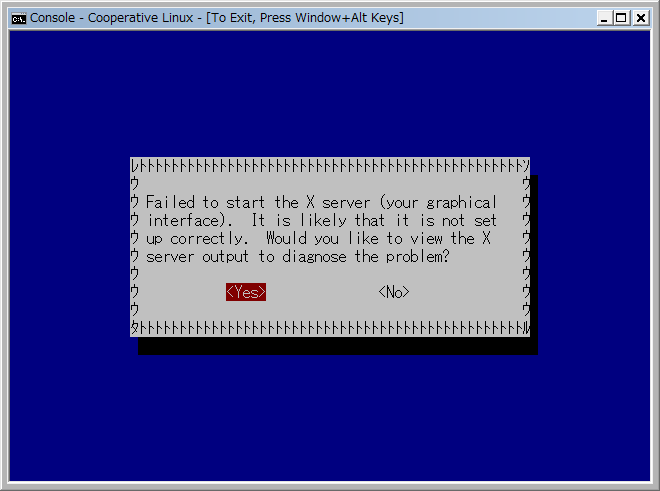
\includegraphics[width=100mm]{image200808/colinux_gdmerror.png}
 \end{center}
 \caption{ターミナルに移動}
 \label{fig:colinux_gdmerror}
\end{figure}

エラーが表示されても、問題なく使用できるですが余り気持ちの良いものではないため、
GDMのインストールが完了したらすぐに、GDMが起動しないように設定します。

/usr/share/gdm/defaults.confを以下のように書き換えます。
\begin{commandline}
   [servers]
-  0=Standard
+  #0=Standard
\end{commandline}

次に/etc/gdm/gdm.confを以下のように書き換えます。
\begin{commandline}
   [xdmcp]
+  Enable=true
\end{commandline}

設定がうまく行えたことを確認するため、
一旦Debianを再起動し、エラーが表示されないことを確認します。

\subsubsection{sshのXフォワードで起動する}
Xmingには、XLaunchというXmingを指定した設定で起動するためのツールが附属しています。
ここではXLaunchを使用して起動してみたいと思います。
まずXLaunchを起動すると、図\ref{fig:colinux_xlaunch}のようなDisplay setting画面が起動されます。
\begin{figure}[htbp]
 \begin{center}
  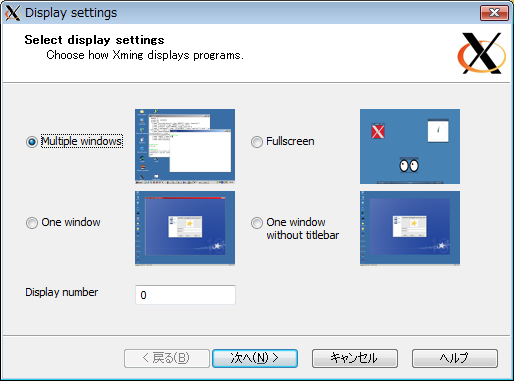
\includegraphics[width=100mm]{image200808/colinux_xlaunch.png}
 \end{center}
 \caption{XLaunch起動}
 \label{fig:colinux_xlaunch}
\end{figure}

起動方法が4種類あるのですが、表\ref{tab:display_setting}のような種類があります。
\begin{table}[htbp]
\begin{center}
  \begin{tabular}[htbp]{|l|l|}\hline
    モード & 表示方法\\ \hline\hline
    Multiple window & 起動するアプリケーション毎にwindowが起動します\\ \hline
    Fullscreen & X Window Systemがフルスクリーンで起動します。\\ \hline
    One window & 1つのwindowにX Window Systemが起動します\\ \hline
    One window whithout titlebar & One windowと同様ですが、タイトルバーが表示されません\\ \hline
  \end{tabular}
  \caption{ディスプレイ設定の選択}
  \label{tab:display_setting}
\end{center}
\end{table}

FullscreenやOne windowはXDMCPでも起動できますので、
ここではMultiple windowで起動してみます。

Multiple windowを選択して「次へ」を選択すると、
Session type画面が表示され、セッションタイプについて聞かれますので、
SSHを使用するStart a programを選択して「次へ」を選択します。
\begin{figure}[htbp]
 \begin{center}
  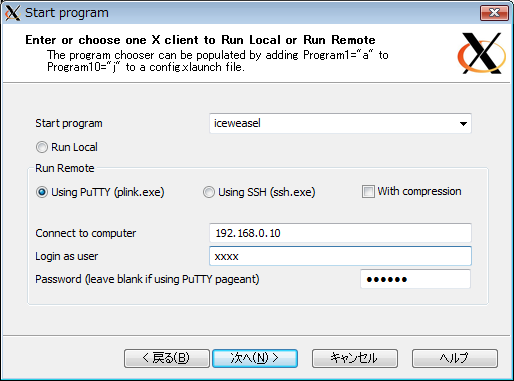
\includegraphics[width=100mm]{image200808/colinux_xlaunch_program.png}
 \end{center}
 \caption{XLaunch起動}
 \label{fig:colinux_xlaunch_program}
\end{figure}

すると図\ref{fig:colinux_xlaunch_program}のようなStart program画面が表示されますので、
Start programに起動するXアプリケーションを指定します。
ここではiceweaselを起動するため、iceweaselと入力します。
Using PuTTY(plink.exe)を選択し、Connect to computerにcoLinuxのIPを入力します。
coLinuxの名前解決ができるようであればホスト名を入力しても問題ありません。
Login as userにユーザ名を入力し、パスワードを入力し、「次へ」を選択します。

Additional parameters画面が表示されますが、
特に指定する必要はありませんので、そのまま「次へ」を選択します。

Finish configuration画面が表示されますので、
「完了」を選択すると、iceweaselが起動します。
「Save configuration」を選択すると、今回行った設定を保存することができます。
Include PuTTY Password as insecure clear textにチェックを入れると、
設定ファイルにパスワードを保存することができますが、
平文で保存されますので注意が必要となります。

保存された設定ファイルをダブルクリックすると、
Xmingが起動され、sshで接続を行い、iceweaselを簡単に起動することができるようになります。

\subsubsection{XDMCPで起動する}
XDMCPの起動では、表\ref{tab:display_setting}のモードの内、
Multiple window以外の起動方法で表示することができます。
ここではOne windowで起動してみます。

XLaunchを起動し、Display setting画面にてOne windowを選択して「次へ」を選択すると、
Session type画面が表示され、セッションタイプについて聞かれますので、
Open session via XDMCPを選択して「次へ」を選択します。
\begin{figure}[htbp]
 \begin{center}
  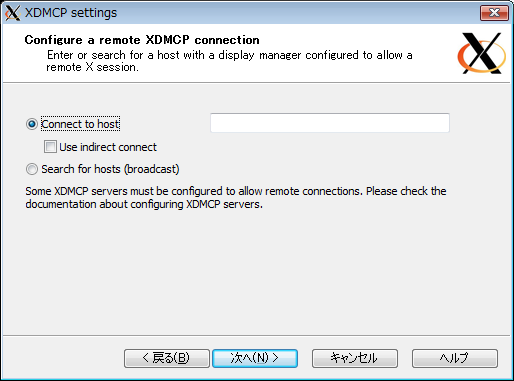
\includegraphics[width=100mm]{image200808/colinux_xlaunch_xdmcp.png}
 \end{center}
 \caption{XLaunch起動}
 \label{fig:colinux_xlaunch_xdmcp}
\end{figure}

すると図\ref{fig:colinux_xlaunch_xdmcp}のようなXDMCP setting画面が表示されますので、
Connect to hostにcoLinuxのIPアドレスを入力します。
coLinuxの名前解決ができるようであればホスト名を入力しても問題ありません。
Additional parameters画面が表示されますが、
特に指定する必要はありませんので、そのまま「次へ」を選択します。

Finish configuration画面が表示されますので、
「完了」を選択すると、GDMが起動し、ログイン画面が表示されます。

「Save configuration」を選択すると、今回行った設定を保存することができます。
ログインが完了すると、GNOME環境が起動しますので、
Application→Internet→Iceweasel Web Browserを選択し、iceweaselを起動します。

以上駆け足でしたが、coLinuxにDebianを新規インストールしたり、
ディスプレイデバイスを持たないcoLinuxでのXアプリケーションの起動について紹介いたしました。

\dancersection{今後の予定}{山下 尊也}

\subsection{次回}
次回は、2008年9月中旬に第17回 関西Debian勉強会を開催する予定です。

\subsection{KDRのおしらせ}
関西Debian勉強会の有志で
関西Debian勉強会とは独立した形で、
週に一度、読書会(KDR)を開いています。
詳しくはKDR公開用ページ\footnote{\url{http://qwik.jp/kdrweb/}}
をご覧下さい。

\dancersection{メモ}{}

\mbox{}\newpage

\printindex
 \cleartooddpage

 \begin{minipage}[b]{0.2\hsize}
  \rotatebox{90}{\fontsize{80}{80} {\gt 関西デビアン勉強会} }
 \end{minipage}
 \begin{minipage}[b]{0.8\hsize}

 \vspace*{15cm}
 \rule{\hsize}{1mm}
 \vspace{2mm}
 
\includegraphics[width=2cm]{image200502/openlogo-nd.eps}
 \noindent \Large \bf Debian 勉強会資料\\ \\
 \noindent \normalfont \debmtgyear{}年\debmtgmonth{}月\debmtgdate{}日 \hspace{5mm}  初版第1刷発行\\
 \noindent \normalfont 関西 Debian 勉強会 (編集・印刷・発行)\\
 \rule{\hsize}{1mm}
 \end{minipage}

\end{document}
